% !TeX spellcheck = en_US
\documentclass[./main.tex]{subfiles}
\begin{document}

\section{Relevant links}

\begin{itemize}
	\item \href{https://github.com/commed-it/backend}{GitHub backend}
	\item \href{https://github.com/commed-it/docs}{GitHub docs}
	\item \href{https://github.com/orgs/commed-it/projects/1}{GitHub project}
	\item \href{https://drive.google.com/drive/folders/15iM-Fm6krEBcHkVyaqSUfjJMY1MKBMm6?usp=sharing}{Slides of the presentation}
	\item \href{https://docs.google.com/spreadsheets/d/1qyKpYXf7lZ2p7q09JHzv7e7yGVBiPEqGNHhwPsFYcXc/edit?usp=sharing}{Spreadsheet documentation}
\end{itemize}

\section{Planification}

\subsection{User Stories}

The first thing that was done regarding the planification of the project
was to define the behavior of the application in a list of user stories.
The next list exposes all of the actions that the user can do with it as
well as different ways of interacting with it.

\begin{itemize}

\item
  \textbf{US1:} As a guest, I want to register in the application
\item
  \textbf{US2:} As a user, I want to log in to the application.
\item
  \textbf{US3:} As a registered user, I want to create a profile of my
  company.
\item
  \textbf{US4:} As a guest, I want to search for services or products so
  that I receive said list.
\item
  \textbf{US5:} As a guest, I want to have a detailed view of the
  product/service.
\item
  \textbf{US6:} As a registered user who has a company profile, I want
  to create services/products.
\item
  \textbf{US7:} As a user, I want to be able to \emph{connect} with a
  company that has made a publication.
\item
  \textbf{US8:} As a user, I need to be able to speak in a chat with the
  company that I connected.
\item
  \textbf{US9:} As a company, I want to respond in the chat with the
  users that have sent messages.
\item
  \textbf{US10:} As a company, I want to send a Formal Offer which
  contains a contract as a PDF through the chat.
\item
  \textbf{US11:} As a company, I want to digitally sign contracts.
\item
  \textbf{US12:} As a user, I want to digitally sign contracts.
\item
  \textbf{US13:} As a user, I want to receive evidences of the process
  when a contract is signed.
\item
  \textbf{US14:} As a user, I want to receive billing and invoices
  regarding the signed commercial transaction contract.
\end{itemize}

\hypertarget{sprint-1}{%
\subsection{Sprint 1}\label{sprint-1}}

The next step was creating a Scrum Board inside a Github project with
the following structure:

\begin{figure}[h]
\centering
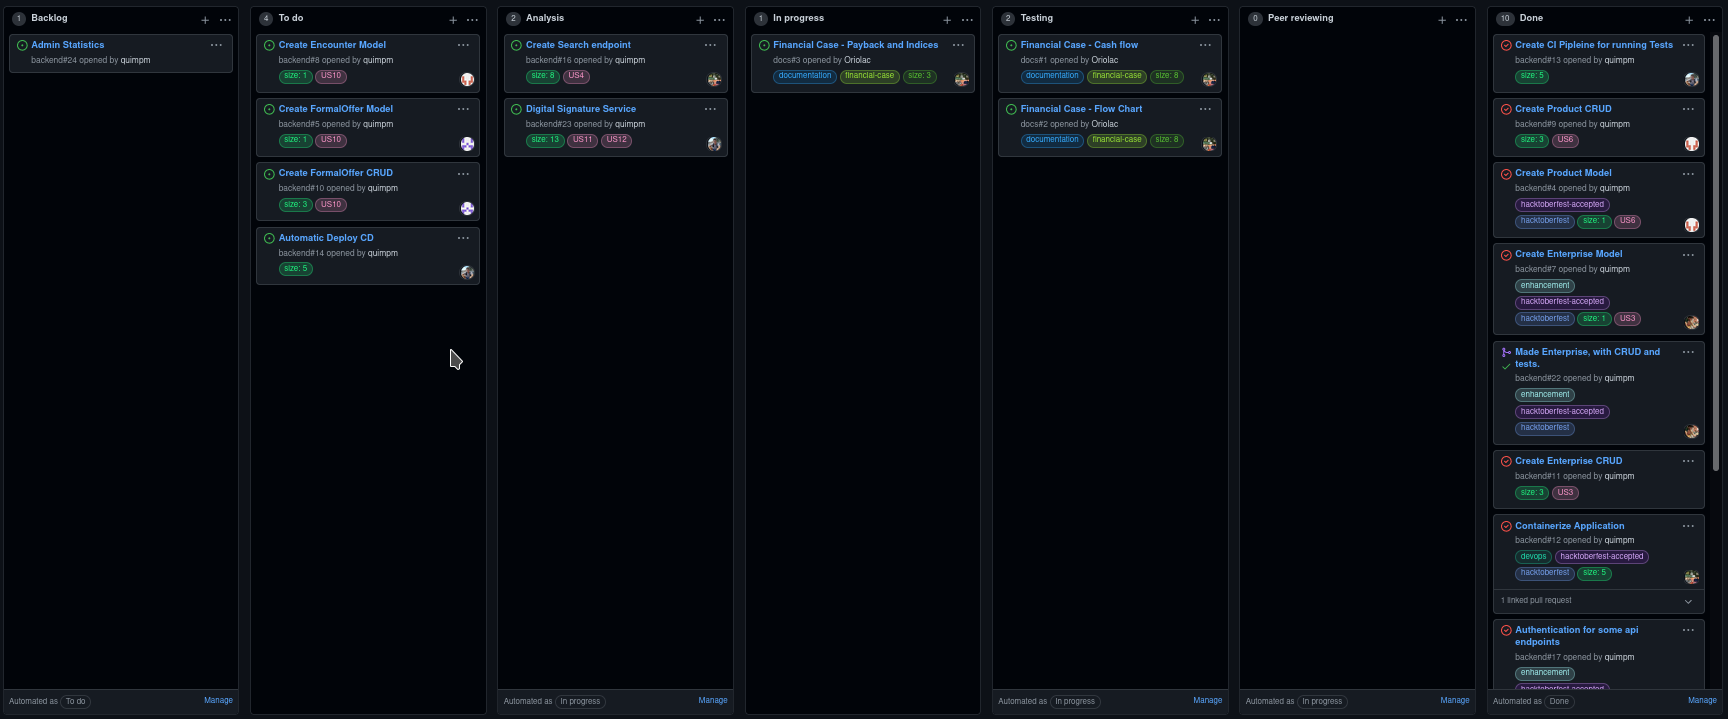
\includegraphics[width=\linewidth]{img/scrum_board.png}
\caption{Github project sceen}
\end{figure}
Afterwards, a meeting was held in order to fulfill the product backlog
with all the tasks that had to be done. These tasks were related to User
Stories, but they were divided so that the product backlog had a small
granularity in the given tasks.
\\
\\
Later, all the tasks were described as a list of things to implement.
Additionally, a weight was given for the complexity of the task and
said weight has to be a number on the Fibonacci Sequence.
\\
\\
After that, all the tasks that had to be done in the First Sprint were
moved in a \emph{To Do} column in the project, which was the name that
was given to the commonly said \textbf{Sprint Backlog}.
\\
\\
Finally, all of the tasks were self assigned, depending on how every
member of the team wanted to contribute. By having each member choose
their own work, it makes it easier to stay motivated.
\\
\\
Sprint 1 Backlog:
\begin{verbatim}
- Configure DB
    - size: 2
- Configure Swager
    - size: 3
- Authentication for some API endpoints
    - size: 8
    - US1, US2
- Conteinarize Aplication:
    - size: 5
- Create Enterprise Model
    - size: 1
    - US3
- Create Enterprise CRUD
    - size: 3
    - US3
- Create Product Model
    - size: 1
    - US6
- Create Product CRUD
    - size: 3
    - US6
- Create CI Pipeline for running tests
    - size: 5
- Financial Case - Cash Flow
    - size: 8
- Financial Case - Flow Chart
    - size: 8
- Financial Cas - Payback and Indices
    - size: 3
- Create Search endpoint
    - size: 8
    - US4
- Digital Signature Service
    - size: 13
    - US11 US12
- Create Encounter Model
    - size: 1
    - US10
- Create Encounter CRUD
    - size: 3
    - US10
- Create Formal Offer Model
    - size: 1
    - US 10
- Create Formal Offer CRUD
    - size: 3
    - US: 10
- Automatic Deploy CD
    - size: 5
- Admin Statistics
    - size: 8
\end{verbatim}

\section{Requirements - Product}

In this section the list of requirements that the application has to
offer to the user will be detailed:

\textbf{Sprint 1:}

Functional Requirements:

\begin{itemize}

\item
  The application has to let all kinds of users search for products or
  services.
\item
  The application has to let users register into the application.
\item
  The application has to let users log in to the application if they
  have an active account on the system.
\item
  The application has to let users create an enterprise profile if they
  are logged in.
\item
  The application has to let logged users publish products or services.
\item
  The application has to let logged users interested in either a product
  or a service to start a chat with the owner of it.
\item
  The application has to let logged users who are owners of a given
  product to chat with said interested users through a chat.
\item
  The application has to let logged users send a commercial transaction
  contract when an agreement has been reached.
\item
  The application has to let logged users sign a commercial transaction
  contract sent by the owner of a product that they are interested.
\item
  The application has to generate the evidences for both sides of the
  commercial agreement.
\end{itemize}

Non Functional Requirements:

\begin{itemize}

\item
  The application has to be the most usable possible.
\item
  The application has to be compliant and respect the laws that run in
  each country that it's available in.
\item
  The application mustn't have large waiting times for the client.
\item
  The application has to be portable and easy to deploy.
\item
  The application has to be scalable and always leave the code open to
  the possibility of adding new features in the future.
\end{itemize}

\section{Main use cases}

\begin{figure}[h]
\centering
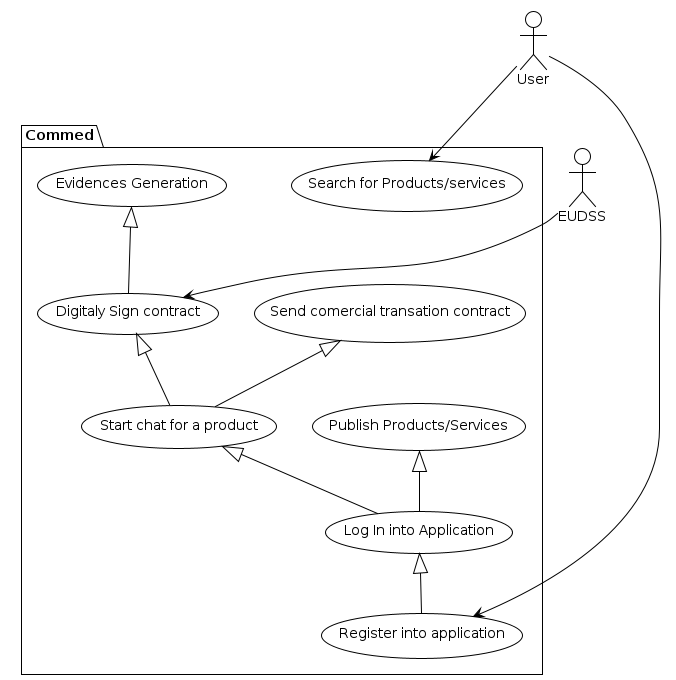
\includegraphics[width=\linewidth]{use_case_diagram/usecase_diagram.png}
\caption{Use case diagram of the application.}
\end{figure}

\begin{itemize}

\item
  \textbf{Register into application}

  \begin{itemize}
  
  \item
    \textbf{Actors:} User
  \item
    \textbf{Purpose:} Let a user register into the application system
  \item
    \textbf{Description:} Provides a screen with a form in which the
    user is able to fulfil it and send the information to the system in
    order to be registered.
  \end{itemize}
\item
  \textbf{Log In into Application}

  \begin{itemize}
  
  \item
    \textbf{Actors:} User
  \item
    \textbf{Purpose:} Log in to the application to be able to use some
    of the application services.
  \item
    \textbf{Description:} Provides a screen with a form in which the
    user will put its email and password. Then, they will log into the
    application so that they can start using the services that it provides.
  \end{itemize}
\item
  \textbf{Search for Products/services}

  \begin{itemize}
  
  \item
    \textbf{Actors:} User
  \item
    \textbf{Purpose:} Search for any product or service the user is
    interested in.
  \item
    \textbf{Description:} Provides a searcher for every user so that
    they can look up the products or services that they are interested
    in.
  \end{itemize}
\item
  \textbf{Publish Products/Services}

  \begin{itemize}
  
  \item
    \textbf{Actors:} User
  \item
    \textbf{Purpose:} Publish services or products in order to be sold
    to other users.
  \item
    \textbf{Description:} Lets a logged user publish the products and
    services that they offer in order for them to be sold to other
    interested users.
  \end{itemize}
\item
  \textbf{Start chat for a product}

  \begin{itemize}
  
  \item
    \textbf{Actors:} User
  \item
    \textbf{Purpose:} Users can start a chat when they are interested in
    a product
  \item
    \textbf{Description:} Lets a logged user start a chat with the
    owners of either a product or a service that they are interested in,
    so that they can start a negotiation.
  \end{itemize}
\item
  \textbf{Send commercial transaction contract}

  \begin{itemize}
  
  \item
    \textbf{Actors:} User
  \item
    \textbf{Purpose:} Send a formal offer with a commercial transaction
    contract.
  \item
    \textbf{Description:} Lets the owners of given products or services
    send a formal offer containing a compliant commercial transaction
    contract within the chat in which the negotiations are taking place.
  \end{itemize}
\item
  \textbf{Digitally Sign contract}

  \begin{itemize}
  
  \item
    \textbf{Actors:} User EUSSD
  \item
    \textbf{Purpose:} Sign a commercial transaction contract sent within
    a Formal Offer.
  \item
    \textbf{Description:} Lets the users of the application sign
    digitally the contract that was sent as a Formal Offer in the chat
    in which the negotiations took place.
  \end{itemize}
\item
  \textbf{Evidences Generation}

  \begin{itemize}
  
  \item
    \textbf{Actors:} User
  \item
    \textbf{Purpose:} Provide users with evidences and the billing of a
    business transaction
  \item
    \textbf{Description:} The system will generate for both parts the
    commercial transaction with all the evidences and the billing of
    the contract.
  \end{itemize}
\end{itemize}

\hypertarget{general-architecture}{%
\section{General architecture}\label{general-architecture}}

\begin{figure}[H]
\centering
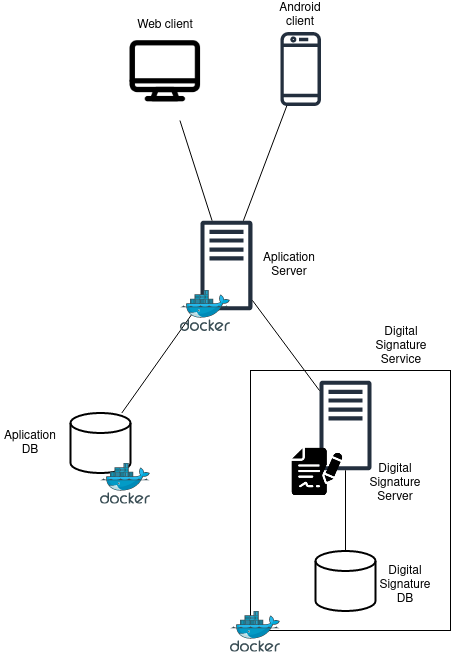
\includegraphics[width=0.6\textwidth]{architecture_diagram/Architecture.drawio.png}
\caption{General architecture of the application.}
\end{figure}
The main item in the architecture is the Application Server. This 
will run in the backend, and furthermore, it will be
responsible for most of the business logic.
\\
\\
This Service will consume resources for another two services. One of
them is its own database, that will be isolated in a single container
and will store all the application data. The other one is the digital
signature service.
\\
\\
As digital signature is a complex thing by itself, it was thought that
it should be isolated in another service, as the whole implementation of
it has nothing related with the business logic held in the Application
Service. So a Digital Signature service with its own database will be
made, isolated in a container in which the Application server will
consume resources.
\\
\\
Finally, the application has two clients that will be consuming
resources from our Application Server. The first one will be the Android
client, which will have the whole user interface. Secondly, a Web client
will be made with a similar user interface, but also administration
pages for the database.
\section{Database model}
The database model can be seen at figure \ref{fig:model-uml}. In the following
sections, it will be reviewed which models shape the application and
which purpose inside the logic do they have.

\begin{figure}[H]
\centering
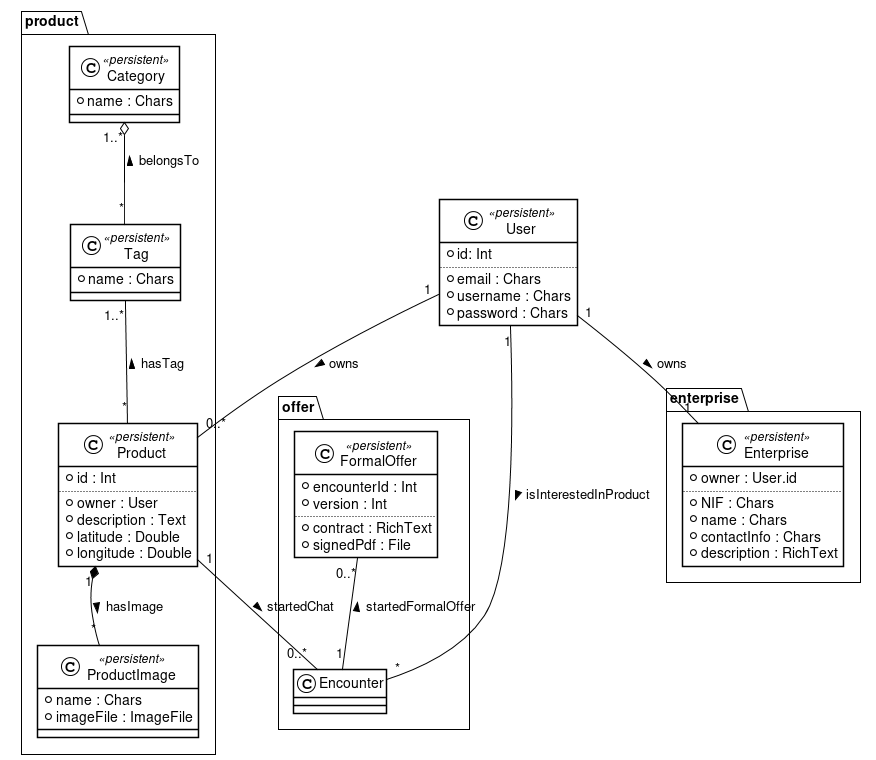
\includegraphics[width=\linewidth]{img/database-model.png}
\caption{UML diagram of the models.}
\label{fig:model-uml}
\end{figure}


\subsection{Users model}
The users model is already provided by Django framework. Its purpose is
to be able to store the usernames and passwords securely. Only
the operations required for the authentication were needed to be done
and not the CRUD operations on the User, based on a JWT Bearer schema.
In \protect\hyperlink{org712facd}{6.1} there is all the explanation
regarding the way that the authentication works.


\subsection{Enterprise Module}
A well known practice inside the Django framework is to separate the
user specific fields in another table instead of extending the User
model. This way, 3\supindex{rd} party apps can be used, for example, for the
authentication part. With this method, not only that the information
such as the enterprise name, description or the fields for generating
its contacts can be stored for a specific user in our app, but
furthermore 3rd party apps that operate on the user can also use it.


\subsection{Product Module}
Each enterprise can post a number of products depending on the plans
that they have subscribed to. This module models the necessary data that
should be stored to do the database.
\\
\\
For the searcher endpoint, a way to categorize the product will be
needed. Because of this, Spacy will be used, which lets us extract keywords and
match against more general tags. For example, it can categorize
``apple'' as ``fruit''. Then, when a client wants to search for a
``pear'', instead of searching against the whole database, it will only
search on the ``fruit'' tag.
\\
\\
To achieve this purpose, we store the tags that are currently used in a
table, and we have a many-to-many relationship between the Product and
Tag table. We made a table for the Tag instead of an enumeration as the
Tag table will be increased programmatically when it encounters a new tag
that does not relate to anything at all.
\\
\\
In the near future and given the fact that the clients won't know about
this inside feature, we will rearrange the tags to minimize the distance
and provide a better support.


\subsection{Formal Offer module}
In this module we will have the models that have the responsibility of
creating formal offers. The most important model is the FormalOffer,
which contains the necessary information to create the unsigned PDF, as
well as the current PDF. It iterates with different versions between the
enterprise that offers the service and the one that wants to buy them,
related to the times the formal offer is sent in the chat. At the end,
the PDF will be agreed upon and signed by both enterprises.
\\
\\
A feature to provide some kind of template in the Formal Offer for the
users was required. The ideal product is to have some kind of Natural
Language Processing service that tries to create a Formal Offer based on
previous formal offers and the messages in the chat. But, this task
required a data to train the model that the application will not have in
the next few years. Meanwhile, the previous contract of the same product
could be given as a template. For this reason, a relation between the
Product model and the FormalOffer model is needed.
\\
\\
The problem is that when the clients start a chat for a product, a
Formal Offer is not created after some time. Additionally, there is no
guarantee that a formal offer will be created for every chat that has
been launched. For this reason, it was decided that creating a model
that has a chat related to them and the product would be better than
storing it in a FormalOffer where all the other values are Null. With
this solution in mind, the Encounter model was created.
\\
\\
\section{Web application}
The administration use case for our application was
done by the Django framework. This can be seen at the screenshots [\ref{fig:admin-1}, \ref{fig:admin-2}, 
\ref{fig:admin-3}, \ref{fig:admin-4}, \ref{fig:admin-5}].
\\
\\
Additionally, some other
form of documentation was provided by the endpoints, including OpenAPI
and swagger docs. This lets the developers have a clear understanding of
what can be done in the API, which will help later on the development of
the Android and the Web application.
\\
\\
The relations in the dashboard are done as shown in the screenshots: the
models are grouped in the application that registered them, and provide
an interface to query, insert, update and delete items in the database.
\\
\\
It was decided that some statistics about the application should be on
the administration tab, but it was left in the backlog for the third
sprint.

\begin{figure}[H]
	\centering
	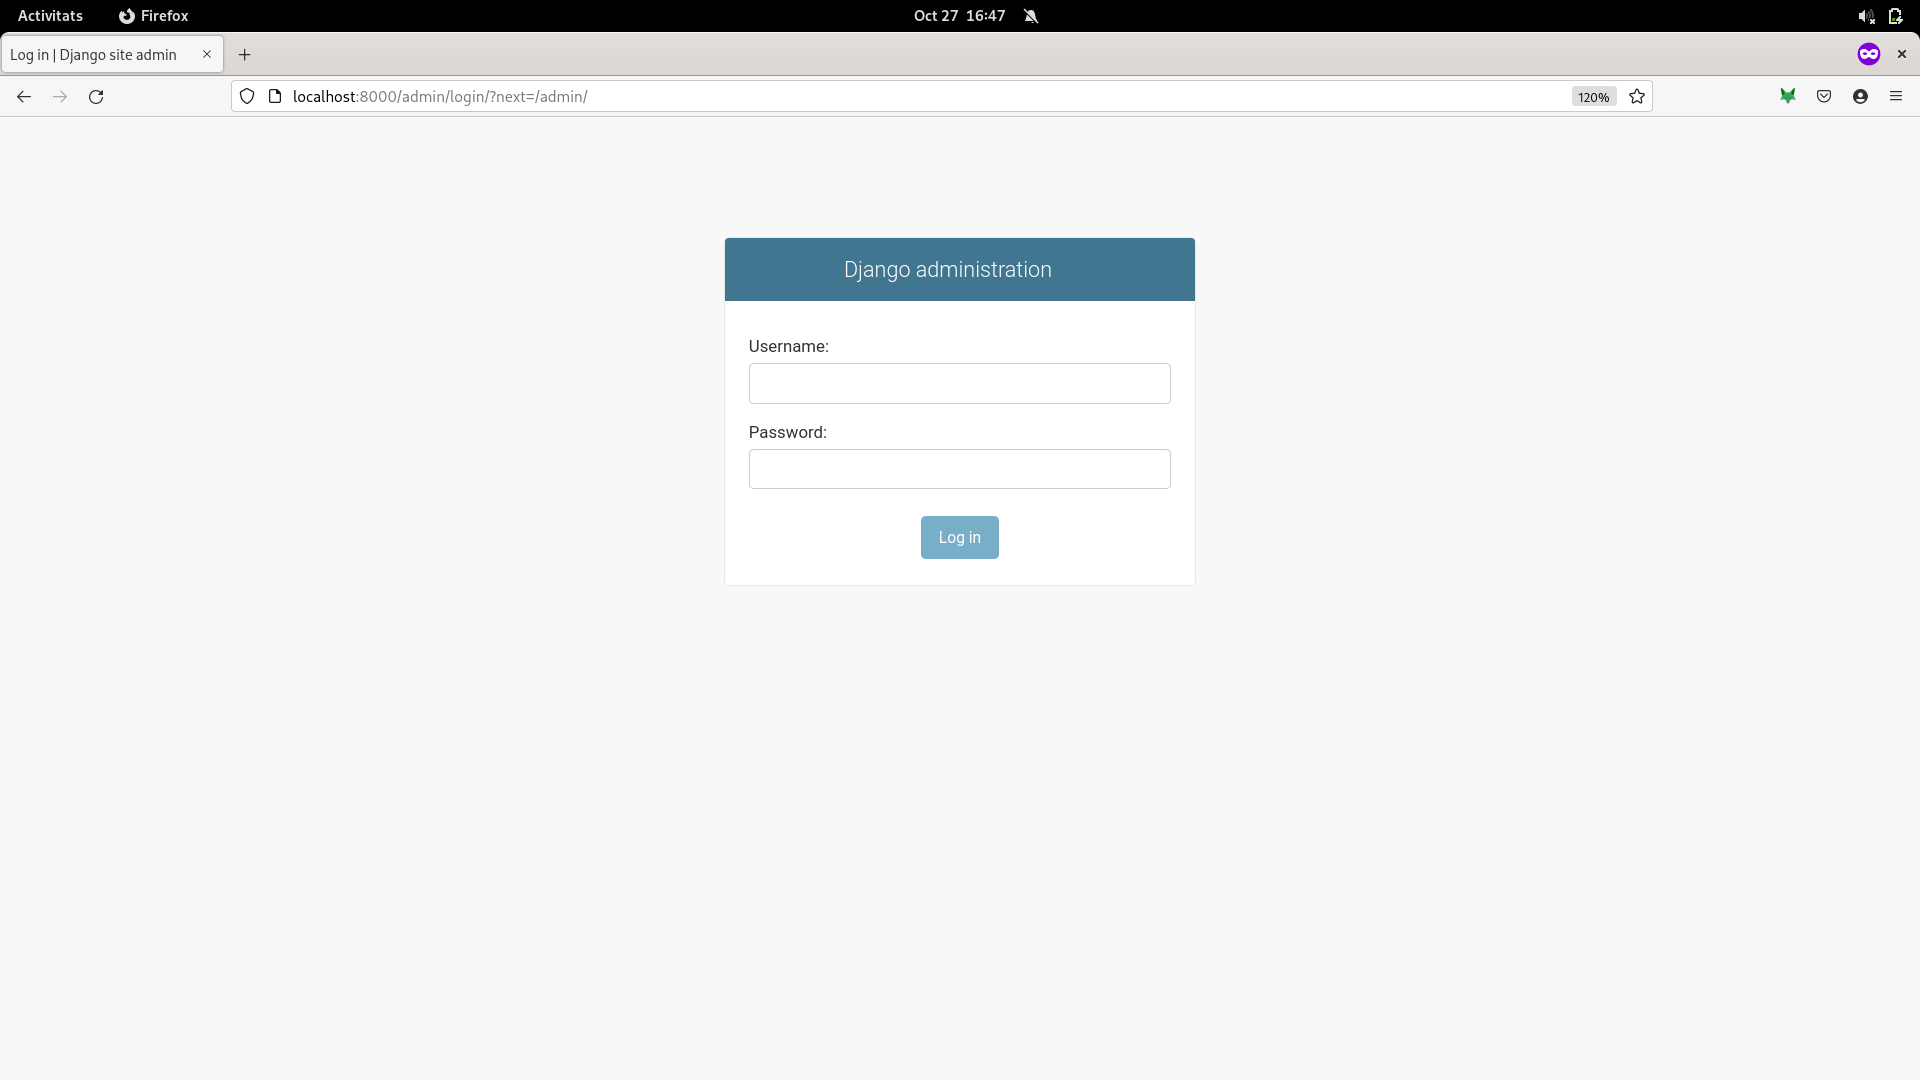
\includegraphics[width=0.9\linewidth]{img/admin-img-1.png}
	\caption{Admin login.}
	\label{fig:admin-1}
\end{figure}

\begin{figure}[H]
	\centering
	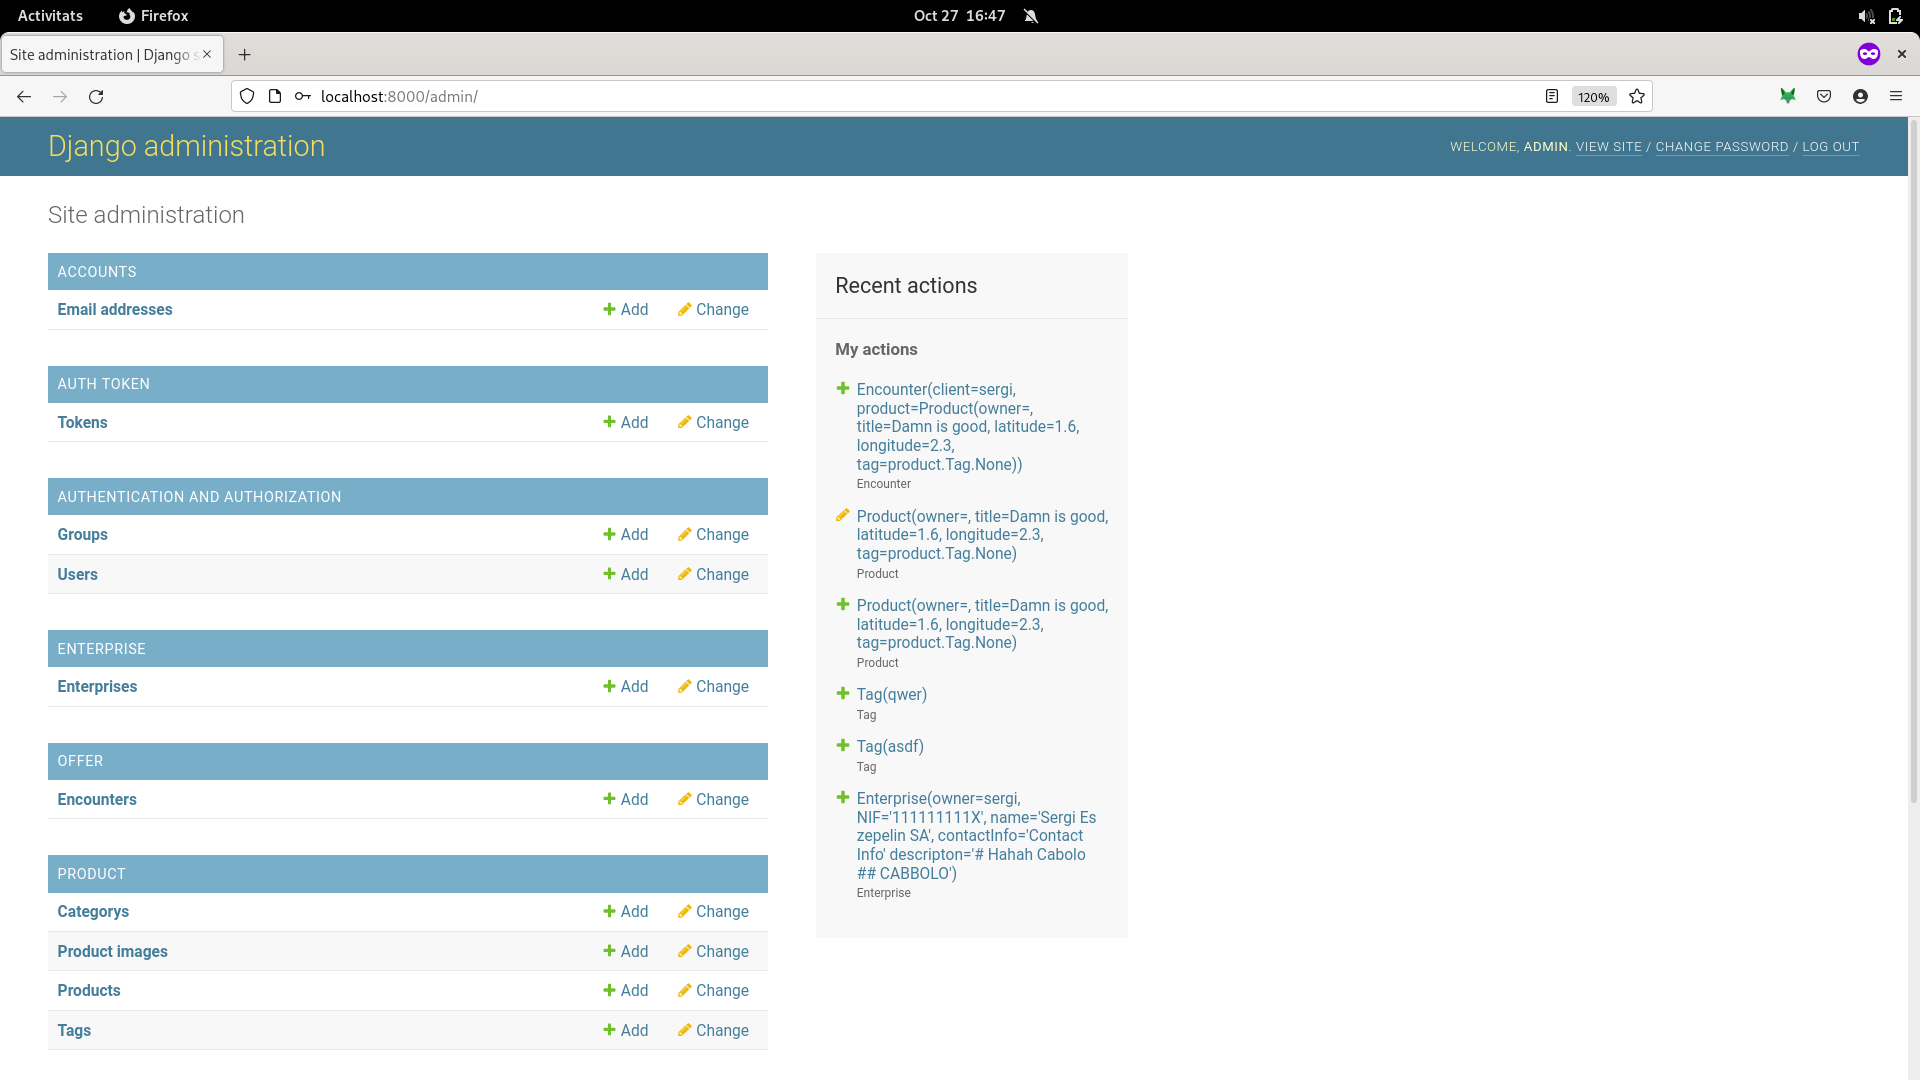
\includegraphics[width=0.9\linewidth]{img/admin-img-2.png}
	\caption{General dashboard. With this you can look all the tables and the last updates.}
	\label{fig:admin-2}
\end{figure}

\begin{figure}[H]
	\centering
	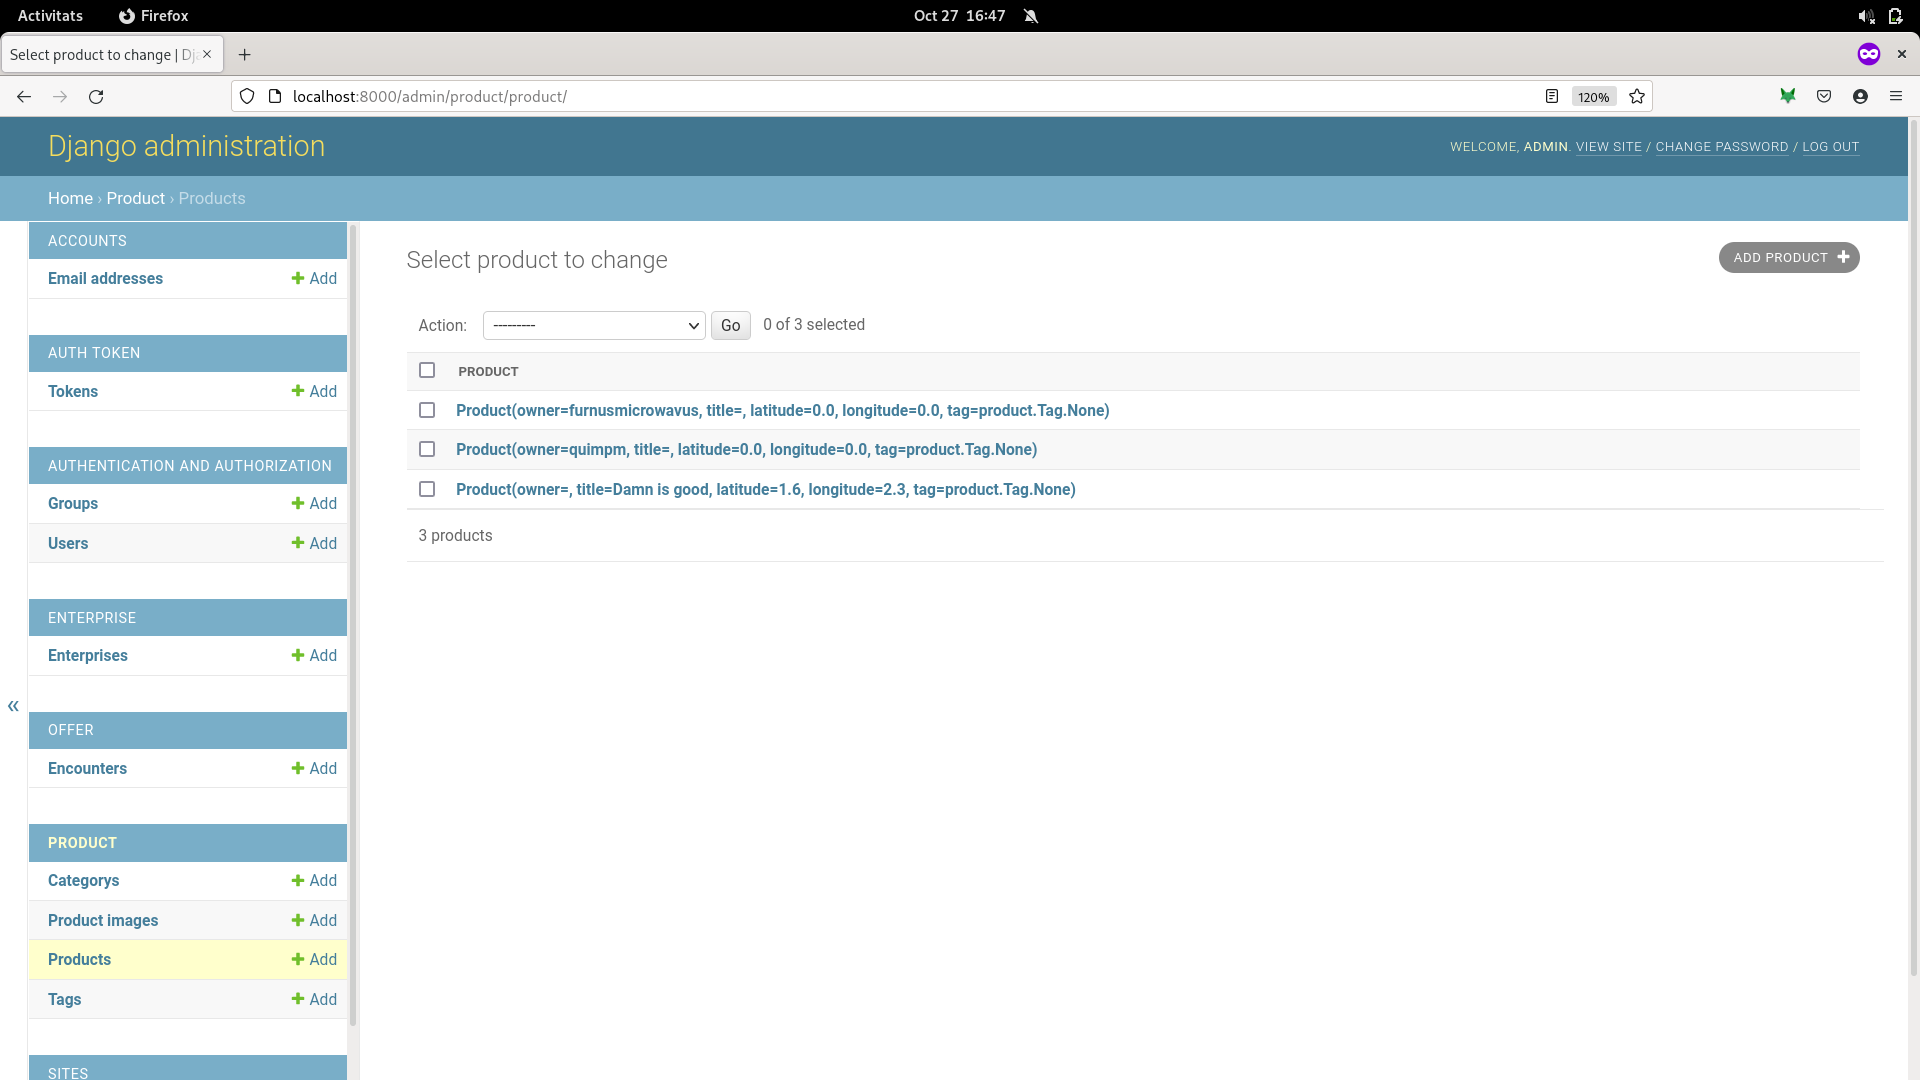
\includegraphics[width=0.9\linewidth]{img/admin-img-3.png}
	\caption{Detail of a Table. In this image , all the records in product can be looked on.}
	\label{fig:admin-3}
\end{figure}

\begin{figure}[H]
	\centering
	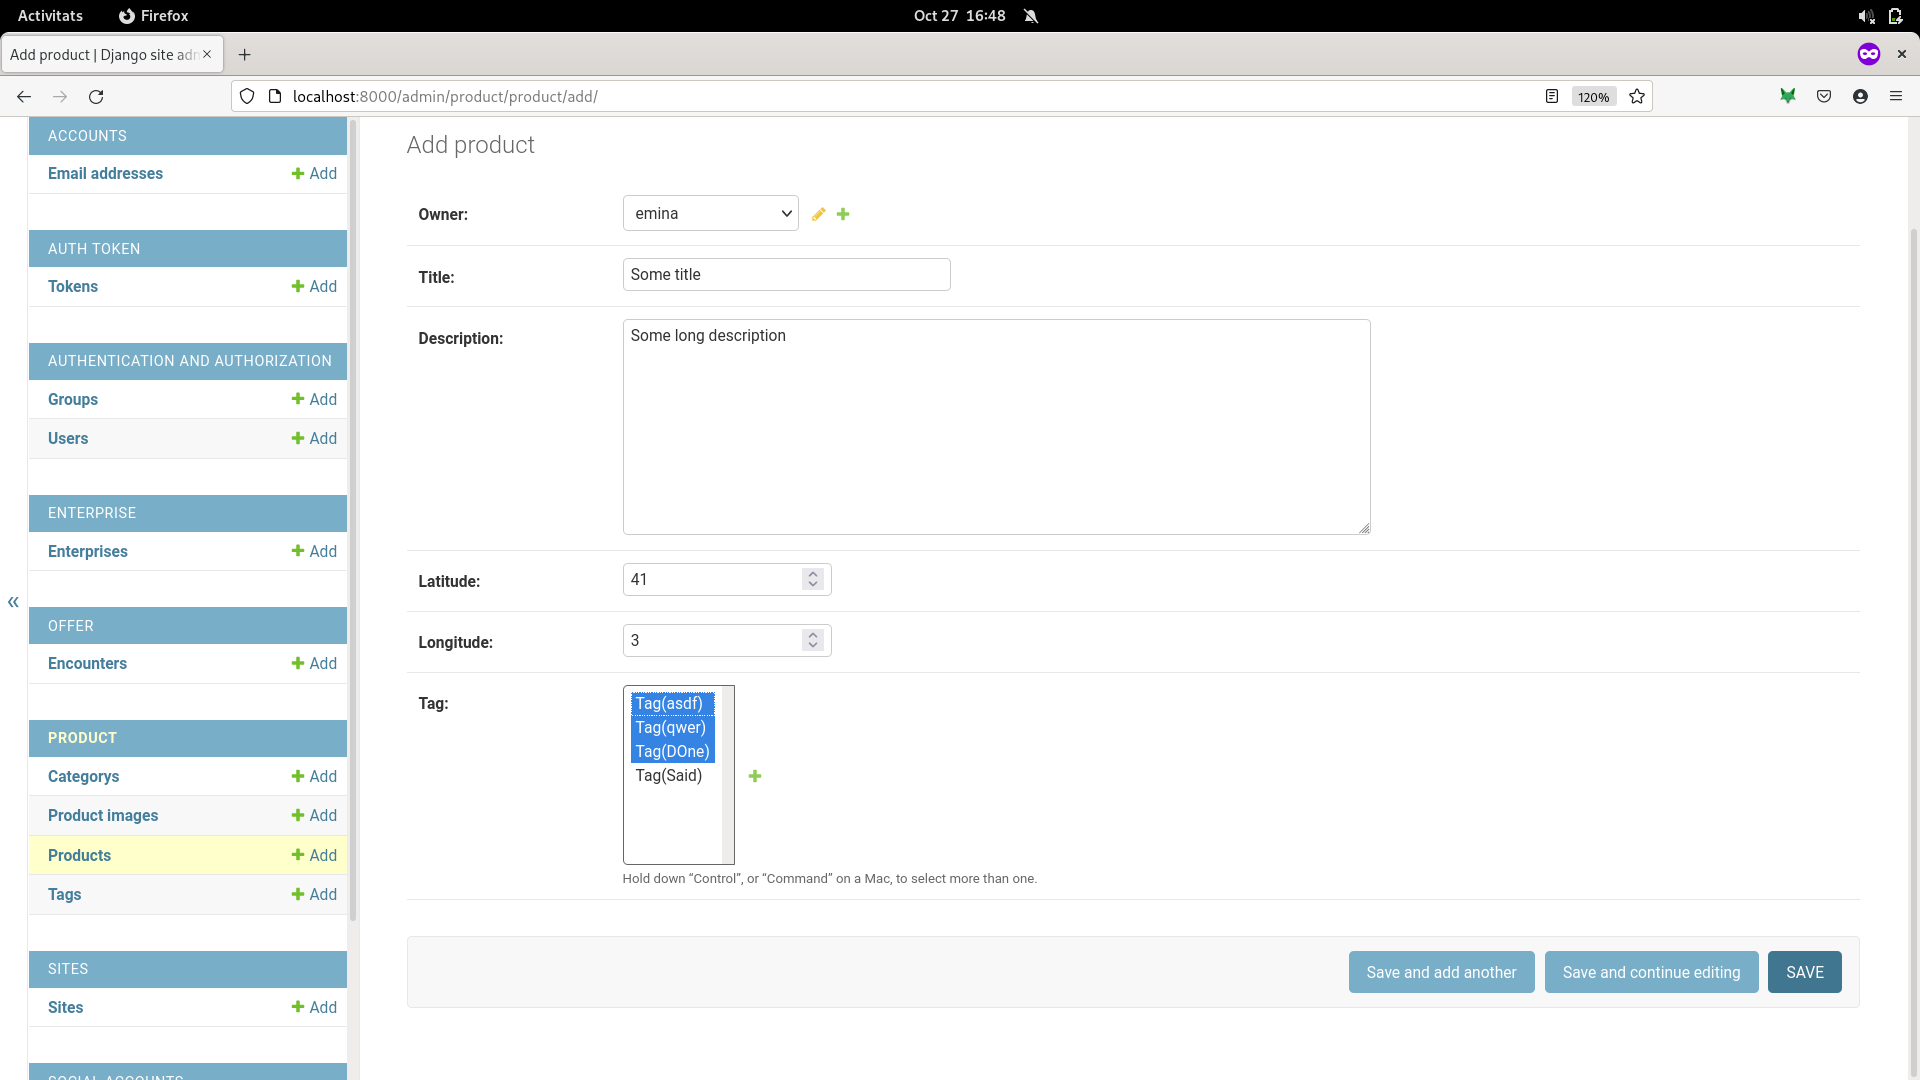
\includegraphics[width=0.9\linewidth]{img/admin-img-4.png}
	\caption{Creation of a product as a form.}
	\label{fig:admin-4}
\end{figure}

\begin{figure}[H]
	\centering
	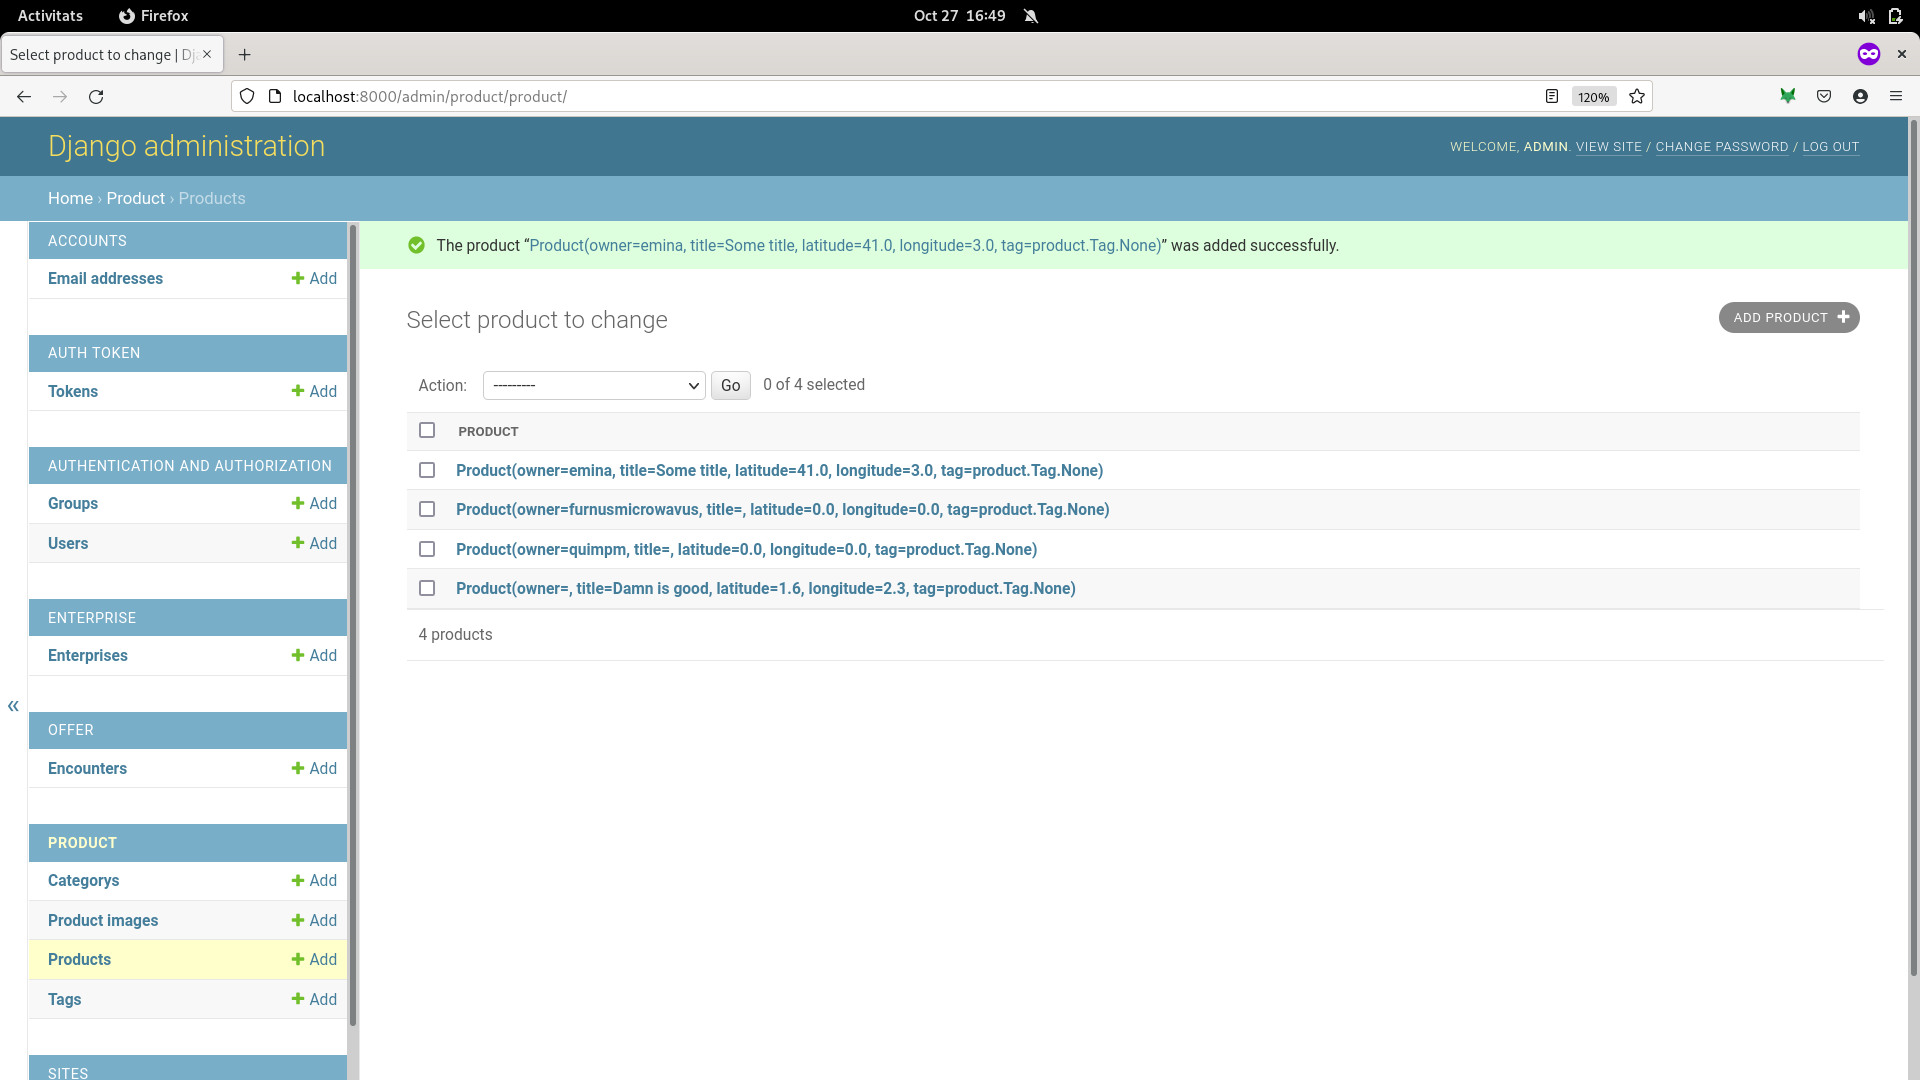
\includegraphics[width=0.9\linewidth]{img/admin-img-5.png}
	\caption{When a record is created, we can see it in the table page along with message.}
	\label{fig:admin-5}
\end{figure}
\subsection{Authentication}

The problem was solved by using two well known apps in the Django
community. The first is maintained by an Enterprise called \emph{IntenCT}
who specializes on doing web applications using Django. This enterprise
published a library that provides an authentication system. It
specializes on keeping users that come from different apps, while
proving a solution for this based on tokens. With this, implementing
simple JavaScript Web Tokens are just a step on the configuration, but
also adding a way to integrate other services for authentication, as a
\textbf{Log In with Google} button use case.\\
\\
The other app that is used provides a REST entrypoint for the first one.
In this way, with just a small configuration a ready-to-go service is
achieved.


\end{document}
